\documentclass[11pt,a4paper]{article}
\usepackage[T1]{fontenc}
\usepackage{lmodern}
\usepackage[margin=25mm]{geometry}
\usepackage{amsmath,amssymb,array,booktabs,tabularx,microtype}
\usepackage{graphicx,float}
\usepackage[authoryear,round]{natbib}
\usepackage[hidelinks]{hyperref}
\newcolumntype{L}{>{\raggedright\arraybackslash}X}
\newcolumntype{P}[1]{>{\raggedright\arraybackslash}p{#1}}
\newcommand{\doi}[1]{\href{https://doi.org/#1}{doi:\nolinkurl{#1}}}
\newcommand{\CO}{CO$_2$}
\newcommand{\clip}{\operatorname{clip}}
\newcommand{\rnd}{\operatorname{round}}
\newcommand{\tablefont}{\small\renewcommand{\arraystretch}{1.14}}
\setlength{\emergencystretch}{1.6em}
\setcounter{topnumber}{3}
\renewcommand{\topfraction}{0.90}
\renewcommand{\textfraction}{0.10}
\raggedbottom

\title{Critical for whom? Choosing scenarios for closer review in power-system flexibility studies}
\author{Th\'eotime Coudray \and St\'ephane Goutte}
\date{19 November 2026}
\begin{document}
\maketitle

\begin{abstract}
Cold, still weather can raise electricity demand just as wind generation falls. Planners simulate such days to see how generation, storage and imports could meet demand. Which scenarios deserve closer review? We assess operating plans from five perspectives. Four give priority to serving demand, controlling costs, limiting direct emissions or obtaining a plan quickly. The fifth weighs these concerns equally. With two minutes to compute each plan, the five perspectives agreed on 48 of their 60 choices from 600 scenarios. Identifying these cases in advance proved harder. On 400 new scenarios, even the best forecast missed more than half the priority cases. We also examined 30 days on one grid. The six days with the highest demand left after wind and solar included some days prioritised for emissions and none of those prioritised for avoidable costs. A planning authority choosing days for review should therefore test its selection rule against the outcome it wants to investigate.
\end{abstract}
\noindent\textbf{Keywords:} power-system flexibility, scenario selection, electricity planning, decision support

\section{Introduction}

Electricity demand and renewable generation follow different rhythms. Solar output can fall late in the day while households are still using electricity. A power system can respond by increasing output from other plants, drawing on stored energy, importing power or shifting some consumption to a later hour. Its ability to adjust supply and demand in this way is called \emph{flexibility} \citep{lannoye2012,ulbig2015}. What the system needs depends on when and where these changes occur. Climate change can shift the season of peak demand, while the mix of wind, solar, storage and transmission determines which adjustments are available \citep{wenz2017,heggarty2019,brown2018}.

Planning authorities use scenarios to explore those possibilities. A scenario describes a particular electricity system and the conditions it faces over a period of time. Analysts might, for example, study an evening with little wind on a network with limited imports. Using a model, they calculate an \emph{operating plan} that specifies which plants generate, when storage charges or discharges, and how power moves between areas. Repeating the exercise for different networks, technologies and weather conditions produces many plans to examine. The European methodology for assessing flexibility needs distinguishes several reasons for examining them, including the integration of renewables and the ability to adjust output as demand changes \citep{acer2025}.

Which scenarios merit a closer look depends on the purpose of that review. Consider a plan that supplies every customer by running thermal plants through the evening. A team responsible for continuity of supply would see its immediate requirement met. A climate analyst might flag the same plan because of the emissions per unit of electricity supplied. An economist would want to know whether another feasible plan could have served the same system more cheaply. The team running the simulations may also flag a case if obtaining a plan takes nearly all the time available. A planning panel might ask how the case fares across all four concerns. These are different questions about a shared result, and one organisation may need to ask several of them.

Existing work gives planners ways to describe the flexibility available in a system \citep{papaefthymiou2018}, to elicit stakeholders' priorities for energy scenarios \citep{voegele2023,hofer2020}, and to select periods that retain important extremes while reducing the work of simulation \citep{hilbers2019}. Here the team must decide which cases to investigate before it knows how their plans will turn out. Characteristics such as the number of areas connected by the grid are already known. Whether a satisfactory plan can be found in time also depends on the scheduling method \citep{smithmiles2012,knueven2020}. Our question is twofold. \emph{Which scenarios warrant closer review under different priorities? How well can we identify them before calculating an operating plan?} We call a scenario \emph{critical} for a given purpose when the plan falls short on the outcomes that matter for that purpose, or when no usable plan is ready in time.

We first compare the cases the five perspectives single out once the plans are known. We then ask what could have been identified beforehand in two settings. In one, the team compares different power systems. In the other, it studies different days on the same grid, where counting lines and plants tells it little about which day to examine. We also vary the time allowed to find a plan. This lets us ask whether a team with a fixed number of computing hours can obtain more plans that meet both cost and service requirements by giving some cases more time than others.

\section{Methods}
\subsection{From a power system to an operating schedule}
\label{sec:scenario}

To build a scenario, we specify the power plants and storage facilities in each area, together with the transmission lines between areas. We then supply time series for demand, wind and solar availability, and water inflows to hydroelectric reservoirs. These inputs describe what the system has to work with over the period being studied.

We study 600 simulated scenarios, referred to as the \emph{development cases}. Each covers one day and contains between 4 and 170 geographical zones. Six groups, or \emph{families}, provide 100 cases each. Three are selected for low, medium or high values of an initial difficulty index within separate pools of candidate cases. The others emphasise renewables and storage, network structure or the number of operating decisions. Every perspective assesses every case.

The scheduling model seeks the lowest-cost plan that respects the limits on power plants, storage and lines. The operating plan, also called a \emph{dispatch}, specifies how much power to generate, store and exchange, and how much consumption to shift to a later hour. A time-limited calculation can return a feasible plan even when a cheaper one exists. The model combines continuous choices, such as power output, with discrete choices, such as whether to start a plant. This makes it a mixed-integer linear program (MILP). It can leave demand unserved at a penalty, so a schedule that satisfies its constraints can still fall short of the study team's service requirement.

We run the program five times for each case, giving it 5, 10, 30, 60 or 120 seconds. Each run starts afresh. A schedule counts as delivered once it has passed the physical checks and the run has ended within its deadline. This clock measures computing time. Each of these development schedules still covers the same 24 hours.

\subsection{Five ways to judge the same schedule}
\label{sec:profiles}

To measure the effect of changing priorities, we keep the dispatch fixed and vary how we judge it. Each row of Table~\ref{tab:profiles} describes a \emph{profile}, meaning the priority given to a particular question. One planning authority might use several profiles during a single study.

\begin{table}[!htb]\centering\tablefont
\caption{Five illustrative perspectives on an operating schedule. The emissions measure covers direct emissions from thermal generation within the modelled system.}\label{tab:profiles}
\begin{tabularx}{\linewidth}{@{}P{.38\linewidth} L@{}}\toprule
Perspective & Question guiding the review\\\midrule
Grid operator (service) & What share of demand went unserved?\\
System planning economist (cost) & How far did operating cost exceed the best known cost for this case?\\
Climate-policy analyst (emissions) & How much thermal generation did the system use per unit of electricity supplied?\\
Study manager (time) & How much of the available computing time did the run use?\\
Public planning panel (balanced) & Which cases deserve attention when all four consequences carry equal weight?\\
\bottomrule\end{tabularx}
\end{table}

Unserved electricity is measured in megawatt-hours (MWh), cost in euros and computing time in seconds. To combine them we put each of the four outcomes on a scale from zero to one, where larger values indicate worse outcomes. For cost we measure how far the plan exceeds the best feasible cost retained from longer runs on the same case (the \emph{reference cost}). For emissions we measure electricity generated by thermal plants within the system per MWh served, using a common emissions factor for those plants. Appendix~\ref{app:scoring} gives the four scales and their units.

For each perspective, we average the four outcomes with stated weights. The first four perspectives give 60\% to their main concern and divide the rest equally among the other three. The balanced perspective gives each outcome 25\%. These illustrative choices produce five scores for a single schedule. A higher score means higher priority for review. If no valid schedule arrives in time, every perspective assigns the maximum score. The amount of unserved electricity in such a run is unknown.

\subsection{What can be predicted before the calculation?}
\label{sec:indicators}

At the point when a study team chooses which scenarios to examine, it knows the system and the operating conditions. It can count zones or compare peak demand with available generating capacity. It cannot yet see the schedule. We use 22 measurable characteristics, or \emph{indicators}, as clues to the eventual outcome. Twelve describe supply, demand and flexibility resources. Ten describe the size and structure of the scheduling problem. The original \emph{reference index} summarises them in one number, giving the two groups equal weight (Appendix~\ref{app:conventions}).

We use completed development runs to learn which indicators predict high scores for each perspective and whether their importance changes with the deadline. The reviewer's weights express what matters. The forecast learns which features of a case help anticipate that result. We compare the 22 indicators recorded by the scenario generator with 22 related measures read from the scheduling model before it is solved. We also test simpler forecasts. One uses zone count, the number of yes-or-no decisions still to be made, and the fraction of zones with thermal capacity. The six counts in the other forecast are zones, time steps, lines, quantities the model must decide, yes-or-no decisions still open, and operating constraints.

\subsection{How the forecasts are tested and used}
\label{sec:protocol}

At 120 seconds we compare the five lists of 60 cases that would merit review if all 600 outcomes were known. To test what the team could have identified beforehand, we then use forecasts. We divide the 600 cases into five groups of 120, with every family represented in each. We fit the forecast on four groups and test it on the fifth, rotating the test group. All runs from one case stay together \citep{cawley2010,roberts2017}. With 12 reviews available in each group, \emph{recall} is the fraction of its 12 highest-scoring cases that the forecast selects. A separate test withholds an entire scenario family.

We next apply the fitted forecasts to 400 independently generated cases. One group of 100 is drawn directly from the scenario generator, without first selecting for difficulty. The other three change the operating period or time resolution, the layout of the network, or how storage power, storage duration and the shape of demand vary together. We measure score accuracy by the average squared difference between forecast and observation (\emph{mean squared error}). For a predicted probability of success, the same calculation against the observed zero or one is called the \emph{Brier score} \citep{gneiting2007}. Smaller values indicate more accurate forecasts. Appendix~\ref{app:validation} distinguishes the tests planned in advance from later checks.

To test whether the same forecasts can help choose days on one grid, we keep a 56-zone network, its generators and its initial storage levels fixed. We vary hourly demand and the availability of wind and solar over 30 synthetic days. For each day we start two separate runs, one with 30 seconds and one with 120 seconds to return a plan. A third, longer run provides that day's reference cost. From the information available before each run, we select six days for each priority. Once the plans are known, we compare the mean score of our six choices with that of the six highest-scoring days. We also count how many days the two lists share. Appendix~\ref{app:fixeddays} describes the rules and the comparison with random selection.

Finally we ask how a team should share a fixed amount of computing time to deliver as many acceptable schedules as possible. A schedule meets the \emph{cost requirement} (E) if it arrives on time and its cost overrun stays within 5\% of the absolute reference cost. For reference costs within one euro of zero, we allow an overrun of one euro. The \emph{joint requirement} (ES) also limits unserved energy to 0.001 MWh. We assign a deadline to each case using its predicted chance of meeting both requirements, then count how many of the schedules at those deadlines actually succeed. Giving each case the same time provides the comparison.

\section{Results}

\subsection{How much can reviewers learn from a short run?}

Reviewers need a schedule before they can examine its cost, its emissions or the demand it leaves unserved. With five seconds per case, the model returned a valid schedule for only 132 of the 600 development cases (Figure~\ref{fig:delivery}). Each of the other 468 cases received the highest possible score under all five priorities. For those runs, the score records a missed deadline. No plan is available from which to measure unserved electricity or emissions.

\begin{figure}[!htb]
\centering
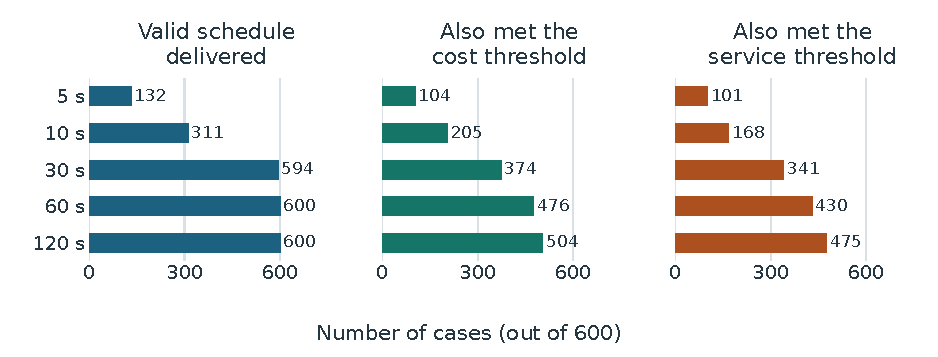
\includegraphics[width=.94\linewidth]{figures/vt_deadline_outcomes.pdf}
\caption{What reviewers can assess at each deadline. The first panel counts valid schedules returned on time. The second counts how many of those meet the cost requirement. The third counts how many also meet the service requirement. Each panel covers the same 600 development cases.}
\label{fig:delivery}
\end{figure}

With 30 seconds, 594 cases returned a valid schedule. With two minutes, all 600 did. Even then, only 475 met both the cost and service requirements. Having a schedule for every case makes it possible to ask which aspects of its performance deserve closer review.

\subsection{Where do the five priorities agree?}
\label{sec:agreement}

Suppose the review team has room to investigate 60 of the 600 cases. We ranked the same two-minute schedules five ways, giving priority in turn to service, cost, computing time or direct emissions, and then giving all four concerns equal weight. Forty-eight cases appeared on every list. That leaves 12 places on each list for which the choice of priority mattered. Across the five lists, 23 different cases occupied those places.

\begin{figure}[!htb]
\centering
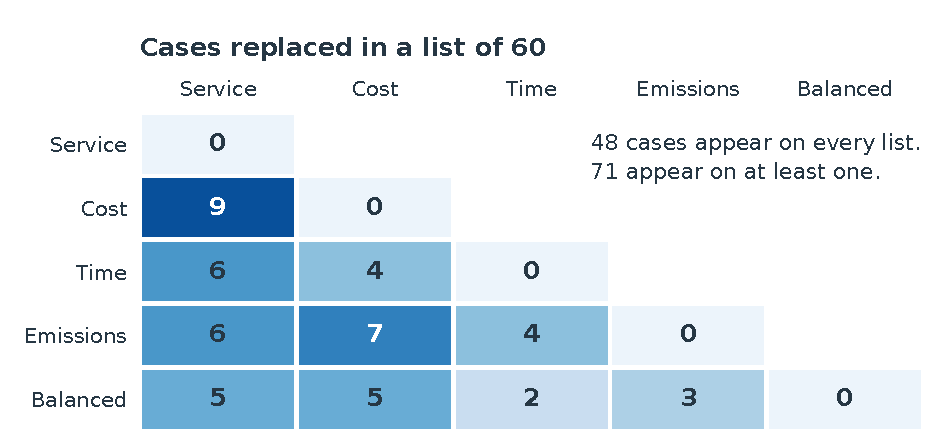
\includegraphics[width=.92\linewidth]{figures/vt_profile_overlap.pdf}
\caption{How many places in a list of 60 change when reviewers switch priorities? Each pair compares the highest-scoring schedules at two minutes. A value of two means that 58 cases stay on the list and two are replaced. All scores use the strengthened cost references.}
\label{fig:profile_overlap}
\end{figure}

The computing-time and balanced lists were closest, sharing 58 cases (Figure~\ref{fig:profile_overlap}). Giving priority to emissions changed three places on the balanced list. One schedule (case D-00020), for example, used 10.9 MWh of internal thermal generation per 100 MWh of demand served. It ranked 51st when emissions had priority, 69th for computing time and 70th with equal weights. It entered only the emissions list.

The largest difference was between service and cost. Of the cases on just one of those two lists, the nine selected for service left a median of 975 MWh unserved, compared with 398 MWh for the nine selected for cost. The latter group exceeded its reference operating cost by a median of 50.7\%, compared with 27.5\% in the service-only group. Figure~\ref{fig:shortlist} in Appendix~\ref{app:switches} shows the individual cases. 

\subsection{Can the priority cases be identified in advance?}
\label{sec:early}

At the start of a study the team knows how the system is configured and what demand it must serve. It has yet to see a schedule. Which of these inputs help anticipate a difficult outcome? On the development cases, the answer changed with the deadline. At five seconds, the share of wind and solar capacity had the largest fitted weight under every priority. With most schedules missing, that association tells us little about the emissions of operating the system. At 30 seconds, the estimated number of discrete operating choices carried the most weight for four profiles. The number of zones mattered most for computing time. At two minutes, thermal units per zone carried about a third of the weight in both the emissions and time forecasts. Allowing weights to change with the deadline reduced forecast error by 24--36\% across the five profiles relative to keeping the same weights and varying only their overall scale. This comparison uses held-out cases from familiar families. Appendix~\ref{app:devfit} reports the results by profile.

A second question is whether a forecast helps choose the cases that experts will review. In each test group we used the forecasts to choose one case in ten for review. We then checked how often those choices matched the cases with the highest observed scores for each priority. Table~\ref{tab:review} compares a forecast trained to predict the score for each priority (the tailored forecast) with one trained on the balanced score. Both use 22 indicators. The last column uses six simple counts of the size of the scheduling problem.

\begin{table}[!htb]\centering\tablefont
\caption{How many priority cases would a reviewer find before the two-minute run? The development test selects 12 cases from each of five groups of 120. The independent test selects ten from each of four groups of 100. Higher counts mean that more of the cases identified in hindsight were selected in advance.}
\label{tab:review}
\begin{tabular}{@{}lrr rrr@{}}\toprule
& \multicolumn{2}{c}{Development (out of 60)} & \multicolumn{3}{c}{Independent (out of 40)}\\
\cmidrule(lr){2-3}\cmidrule(l){4-6}
Review priority & Tailored & Balanced & Tailored & Balanced & Six counts\\\midrule
Service & 28 & 30 & 10 & 10 & 10\\
Cost & 26 & 32 & 7 & 11 & 12\\
Computing time & 37 & 32 & 16 & 13 & 13\\
Direct emissions & 29 & 32 & 9 & 9 & 9\\
Balanced & 33 & 33 & 11 & 11 & 12\\
\bottomrule\end{tabular}
\end{table}

Only the time priority gained cases from tailoring the forecast in both tests. On the independent systems it recovered 16 of the 40 time-priority cases, compared with 13 using the balanced forecast. For service and direct emissions, the two forecasts recovered the same number. For cost, the balanced forecast found more. A panel giving equal weight to all concerns recovered 11 of its 40 priorities with that forecast. Choosing at random would recover four on average. Even the highest count in the independent test leaves more than half of the priority cases unselected. Appendix~\ref{app:selection} examines the cases missed at different review quotas.

\subsection{Which indicators remain informative on new systems?}
\label{sec:final_independent_descriptors}

How well did the system descriptions carry over to the new cases? The six counts, which include the numbers of zones, lines and decisions, are a simple starting point. On the 400 independent cases, these counts gave the smallest average error for all five priority scores among the linear models compared. Here we set forecasts below zero to zero and those above one to one, so they fall on the same scale as the observed scores. For the balanced panel, the six counts also found one additional priority case. For the time-priority list, they found three fewer than the tailored forecast using all 22 indicators. A forecast can therefore estimate scores accurately across the whole sample and still miss cases at the top of the list.

The number of lines per zone illustrates why a forecast can lose accuracy on a new network. The development networks had no loops. In a connected network of this kind (a tree), there is one fewer line than there are zones. The ratio of lines to zones was therefore always below one. Some new grids connected existing zones with additional lines. The model had learned its relationship between network density and the balanced score on trees alone. Applied to the more interconnected grids, it produced scores above six on a scale whose maximum is one (Figure~\ref{fig:transfer} in Appendix~\ref{app:external}). In a later check, limiting this single indicator to its training range removed much of the excess error for the balanced score. Appendix~\ref{app:external} gives that comparison and distinguishes it from the forecasts made before the independent runs.



\subsection{Which days deserve review on the same grid?}
\label{sec:fixeddays}

When planners compare days on an existing grid, the number of zones, lines and plants stays the same. The forecasts using three measures of system structure or six counts therefore gave all 30 days the same score for any given priority and deadline. Yet the plans differed. Day~19, for example, ranked only 19th for peak \emph{residual load}, the demand left after subtracting available wind and solar generation hour by hour. At 30 seconds its plan left 229~MWh unserved, out of 249~MWh across all 30 days. All five perspectives ranked it first for review. At two minutes, a separate run for the same day found a plan that met demand in full. In this case, the missed demand in the first plan could have been served with the resources already on the grid.

Which daily conditions gave a useful warning? Selecting the six days with the highest residual load peaks found three of the six emissions-priority days at 30 seconds and two at 120 seconds. It missed every cost-priority day at both deadlines (Figure~\ref{fig:fixed_grid_days}). Here a day is costly for the reviewer when its plan costs substantially more than another feasible plan for the same day. Even a moderate peak can coincide with such an overrun. The forecast using all 22 measures of the scheduling problem gave each day a different score, yet at two minutes it missed all six priority days under every perspective.

\begin{figure}[!htb]
\centering
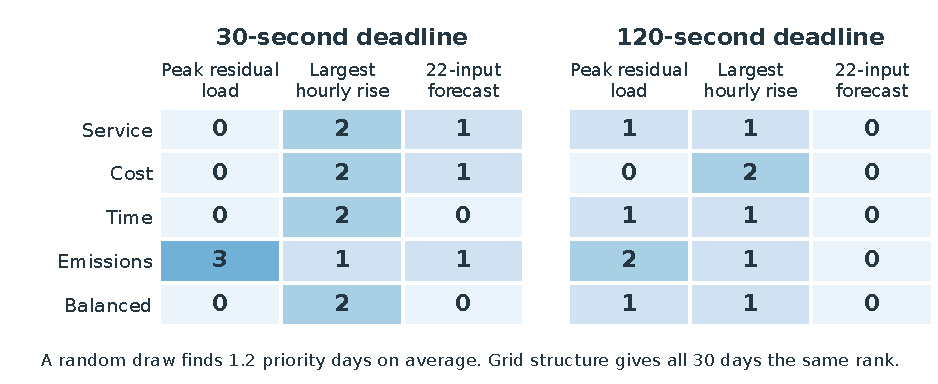
\includegraphics[width=.96\linewidth]{figures/vt_fixed_grid_days.pdf}
\caption{Selecting six days for review on the same grid. Each panel shows how many of the six days with the highest observed score also appeared among a rule's six choices. The peak and hourly rise refer to demand remaining after wind and solar. The 22-input forecast also uses information about the physical system and the hourly operating conditions.}
\label{fig:fixed_grid_days}
\end{figure}

A rule can miss the exact top six and still select days of comparable concern. We therefore also compared the average score of the six days each rule chose. Selecting the days with the sharpest hour-to-hour rise in residual load gave a slightly higher average score than random selection under all five priorities at both deadlines. Each uncertainty interval for this gain included zero (Appendix~\ref{app:fixeddays}). On these 30 days, the evidence for using hourly changes as a screening rule is therefore inconclusive.

\subsection{Can the indicators help distribute computing time?}

We now return to the portfolios that compare different systems. Suppose the team has enough computing time to give each case 30 seconds. Could it obtain more plans that meet both service and cost requirements by giving some cases longer and others less time?

\begin{table}[!htb]\centering\tablefont
\caption{Schedules meeting both service and cost requirements with 30 seconds available per case on average. Uniform allocation gives every case 30 seconds. The next three rules select the deadline from information available before the run. Hindsight shows the most successes attainable if the outcomes at all deadlines were already known.}
\label{tab:allocation}
\begin{tabular}{@{}lrrrrr@{}}\toprule
Cases & Uniform & Zones only & Three indicators & All 22 & Hindsight\\\midrule
Development (600) & 341 & 395 & 413 & 415 & 472\\
Independent (400) & 351 & 352 & 362 & 350 & 374\\
\bottomrule\end{tabular}
\end{table}

On the development cases, the 22 indicators yielded 74 more acceptable schedules than giving every case the same time (Table~\ref{tab:allocation}). A rule based on the number of zones, the estimated number of discrete decisions and thermal units per zone yielded 72 more successes than equal time. On the independent cases, the 22-indicator rule produced one fewer acceptable schedule than equal time. The three-indicator rule still delivered 11 more (paired 95\% interval, 6--18). These new systems also left less room for improvement. Even with full knowledge of the outcomes, only 23 additional schedules could have met both requirements at that reserve. Appendix~\ref{app:reserve} reports how the comparison changes with the time available.

\section{Discussion}

\subsection{What does inclusion on a priority list mean?}

For a public planning panel, the distinction between cases everyone would select and cases selected for a particular reason is useful. The 48 cases common to all five lists give the panel a starting point once it has seen the schedules. The remaining places give it room to examine concerns that an overall ranking can conceal. The schedule in Section~\ref{sec:agreement}, for example, entered the emissions list alone. Publishing the amount of thermal generation per unit of demand served alongside the rank makes that choice intelligible. A panel concerned with the emissions of electricity consumed would also need to account for the origin of imports.

The same principle applies to operating cost and continuity of supply. For an economist, a large excess over the reference cost means that a cheaper feasible schedule exists for the same system and operating conditions. An analyst assessing an investment in storage would still need to compare operation with and without that investment, and to consider market prices and access conditions \citep{newbery2024}. For a grid operator, the physical question is whether there was a way to serve demand. At two minutes, 29 development schedules met the cost requirement but left more demand unserved than the study allowed. For all 29 we found an alternative plan for the same case that met both requirements (Appendix~\ref{app:switches}). Identifying a poor schedule can therefore justify further work on scheduling before an apparent shortage is attributed to the system itself.

The computing-time result matters to the team responsible for delivering the study. At five seconds, a missing plan gave every reviewer the same reason for concern. At two minutes, a tailored forecast helped identify cases that used a large share of the time available. That makes it a candidate for deciding which runs need closer supervision. Deciding which runs should receive \emph{more time} requires checking whether the extra time produces a schedule that meets the agreed requirements. On the independent cases, the simple three-indicator rule improved that outcome, while the full set of 22 offered no gain at the same reserve.

\subsection{Which findings carry over to another study?}

The weights in this study illustrate choices a planning body might make. A decision-making body can choose its own weights or set a condition that every acceptable plan must meet. An equal-weight score allows good performance on one criterion to offset poor performance on another. A binding service threshold rules out that trade-off. In either case, a team using a forecast to select cases could report how many consequential cases it missed in a separate test and show the size of the omissions in physical units. In our independent test, one case missed by the service forecast left 3,501 MWh unserved. That quantity conveys a consequence that the number of missed cases alone cannot.

Our test covers new simulated systems designed with the same modelling tools. Varying network connections and the length of the operating period tests whether relationships learned under familiar conditions still hold when those features change. It gives no estimate of how often a critical situation occurs on a real grid. The model represents regional energy balances and limits on power flows. Assessing voltage, frequency or the consequences of losing a line would require further engineering analysis.

The daily study also shows why a review team needs to look at the quantity behind a rank. On the same 30 days, 22 plans met both the service and cost requirements at 30 seconds and 28 did so at two minutes. At two minutes all 30 plans served demand in full, yet only one day appeared on all five lists of six. Even the service-priority list distinguished among days, because cost, time and emissions still carried some weight. A reviewer investigating potential shortages would learn more at that point by checking the unserved energy directly.

The daily experiment covers one simulated network and one timed run per day and deadline. Other grids and repeated runs under the same operating conditions would help establish how often these rules miss consequential days. The development study also illustrates uncertainty in cost and timing. There, longer reference runs changed one member of the emissions list and left the other four lists intact. In a separate timing check, five of 30 selected development cases met the joint requirements in some two-minute runs and missed them in others. Changes close to a numerical cutoff deserve particular care when they determine whether a case receives further attention.

\section{Conclusions and policy implications}

When an authority commissions a flexibility study, the purpose of the review should guide the choice of scenarios. In the comparison of 600 scenarios at two minutes, most cases chosen for detailed examination warranted attention under all five priorities. The remaining places depended on the question being asked. A list based on equal weights, for example, omitted a case that a climate analyst would have selected for its reliance on thermal generation. Reporting both the common cases and the reason for including additional ones would make the scope of an assessment clearer.

Choosing cases before their schedules are known is harder. At a review quota of one case in ten, even the best forecast in our independent comparison recovered fewer than half the cases reviewers would have selected with hindsight. A rule that helps compare different grids also needs a separate test before it is used to select days on one grid. In our daily study, the largest peaks in demand left after wind and solar identified some days of concern for direct emissions and missed all the priority days for cost. Reporting which days a rule would leave out, and what happened on those days, makes its consequences visible to reviewers. A team with limited computing time can count how many additional schedules meet its requirements when it lets some runs continue longer. An indicator is worth collecting for that decision if it helps produce more acceptable schedules within the time the team has.

\setlength{\bibsep}{0.28\baselineskip}
\begin{thebibliography}{99}
\bibitem[ACER(2025)]{acer2025}
European Union Agency for the Cooperation of Energy Regulators (ACER), 2025.
Type and format of data and the methodology for TSOs' and DSOs' flexibility needs analysis.
Decision No.~05/2025, Annex~I, 25 July.
\href{https://www.acer.europa.eu/sites/default/files/documents/Individual\%20Decisions_annex/ACER-Decision-05-2025-FNAM-Annex-I.pdf}{Flexibility needs assessment methodology}.

\bibitem[Brown et~al.(2018)]{brown2018}
Brown, T., Schlachtberger, D., Kies, A., Schramm, S., Greiner, M., 2018.
Synergies of sector coupling and transmission reinforcement in a cost-optimised, highly renewable European energy system.
\emph{Energy} 160, 720--739. \doi{10.1016/j.energy.2018.06.222}.

\bibitem[Cawley and Talbot(2010)]{cawley2010}
Cawley, G.C., Talbot, N.L.C., 2010. On over-fitting in model selection and subsequent selection bias in performance evaluation.
\emph{Journal of Machine Learning Research} 11, 2079--2107. \url{https://www.jmlr.org/papers/v11/cawley10a.html}.

\bibitem[Gneiting and Raftery(2007)]{gneiting2007}
Gneiting, T., Raftery, A.E., 2007. Strictly proper scoring rules, prediction, and estimation.
\emph{Journal of the American Statistical Association} 102, 359--378. \doi{10.1198/016214506000001437}.

\bibitem[Heggarty et~al.(2019)]{heggarty2019}
Heggarty, T., Bourmaud, J.-Y., Girard, R., Kariniotakis, G., 2019.
Multi-temporal assessment of power system flexibility requirement.
\emph{Applied Energy} 238, 1327--1336. \doi{10.1016/j.apenergy.2019.01.198}.

\bibitem[Hilbers et~al.(2019)]{hilbers2019}
Hilbers, A.P., Brayshaw, D.J., Gandy, A., 2019.
Importance subsampling: improving power system planning under climate-based uncertainty.
\emph{Applied Energy} 251, 113114. \doi{10.1016/j.apenergy.2019.04.110}.

\bibitem[H\"ofer and Madlener(2020)]{hofer2020}
H\"ofer, T., Madlener, R., 2020.
A participatory stakeholder process for evaluating sustainable energy transition scenarios.
\emph{Energy Policy} 139, 111277. \doi{10.1016/j.enpol.2020.111277}.

\bibitem[Knueven et~al.(2020)]{knueven2020}
Knueven, B., Ostrowski, J., Watson, J.-P., 2020. On mixed-integer programming formulations for the unit commitment problem.
\emph{INFORMS Journal on Computing} 32, 857--876. \doi{10.1287/ijoc.2019.0944}.

\bibitem[Lannoye et~al.(2012)]{lannoye2012}
Lannoye, E., Flynn, D., O'Malley, M., 2012. Evaluation of power system flexibility.
\emph{IEEE Transactions on Power Systems} 27, 922--931. \doi{10.1109/TPWRS.2011.2177280}.

\bibitem[Newbery and Biggar(2024)]{newbery2024}
Newbery, D.M., Biggar, D.R., 2024. Marginal curtailment of wind and solar PV: Transmission constraints, pricing and access regimes for efficient investment.
\emph{Energy Policy} 191, 114206. \doi{10.1016/j.enpol.2024.114206}.

\bibitem[Papaefthymiou et~al.(2018)]{papaefthymiou2018}
Papaefthymiou, G., Haesen, E., Sach, T., 2018. Power System Flexibility Tracker: Indicators to track flexibility progress towards high-RES systems.
\emph{Renewable Energy} 127, 1026--1035. \doi{10.1016/j.renene.2018.04.094}.

\bibitem[Roberts et~al.(2017)]{roberts2017}
Roberts, D.R., Bahn, V., Ciuti, S., Boyce, M.S., Elith, J., Guillera-Arroita, G., Hauenstein, S., Lahoz-Monfort, J.J., Schr\"oder, B., Thuiller, W., Warton, D.I., Wintle, B.A., Hartig, F., Dormann, C.F., 2017.
Cross-validation strategies for data with temporal, spatial, hierarchical, or phylogenetic structure.
\emph{Ecography} 40, 913--929. \doi{10.1111/ecog.02881}.

\bibitem[Smith-Miles and Lopes(2012)]{smithmiles2012}
Smith-Miles, K., Lopes, L., 2012. Measuring instance difficulty for combinatorial optimization problems.
\emph{Computers \& Operations Research} 39, 875--889. \doi{10.1016/j.cor.2011.07.006}.

\bibitem[Ulbig and Andersson(2015)]{ulbig2015}
Ulbig, A., Andersson, G., 2015. Analyzing operational flexibility of electric power systems.
\emph{International Journal of Electrical Power \& Energy Systems} 72, 155--164. \doi{10.1016/j.ijepes.2015.02.028}.

\bibitem[V\"ogele et~al.(2023)]{voegele2023}
V\"ogele, S., Teja Josyabhatla, V., Ball, C., Rhoden, I., Grajewski, M., R\"ubbelke, D., Kuckshinrichs, W., 2023.
Robust assessment of energy scenarios from stakeholders' perspectives.
\emph{Energy} 282, 128326. \doi{10.1016/j.energy.2023.128326}.

\bibitem[Wenz et~al.(2017)]{wenz2017}
Wenz, L., Levermann, A., Auffhammer, M., 2017. North--south polarization of European electricity consumption under future warming.
\emph{Proceedings of the National Academy of Sciences} 114, E7910--E7918. \doi{10.1073/pnas.1704339114}.
\end{thebibliography}

\clearpage

\appendix
\section{From dispatch outcomes to scores}
\label{app:scoring}

\paragraph{Profile scores.}
Let \(s=(r,d)\) denote one case, where \(r\) is the physical system and \(d\) its operating conditions. At computing deadline \(b\), let \(L_j\) denote the observed loss for criterion \(j\) when a schedule is delivered. The four criteria are unserved energy (\(U\)), cost (\(C\)), elapsed time (\(T\)) and direct thermal emissions (\(Q\)). Let \(\pi_j^p\) be the weight assigned to criterion \(j\) by decision profile \(p\), using the weights described in Section~\ref{sec:profiles}. The observed profile score \(Y^p_{s,b}\) is
\begin{equation}
 Y^p_{s,b} =
 \begin{cases}
 \displaystyle\sum_{j\in\{U,C,T,Q\}}\pi_j^p L_j, & \text{if a valid schedule for case \(s\) arrives by \(b\)},\\
 1, & \text{otherwise}.
 \end{cases}
 \label{eq:profileloss}
\end{equation}
A run without a schedule receives its score directly, without assigning values to the missing physical outcomes.

\paragraph{Timely physical validation.}
We used HiGHS 1.14.0 with 16 solver threads through Pyomo 6.10.0 on Windows. For each candidate schedule we independently recalculate the cost and check balances, line and equipment capacities, ramp limits, storage and deferred-load balances, and integrality. Absolute tolerances are \(10^{-3}\) in physical checks and \(10^{-5}\) for integer decisions. An overrun, invalid schedule or failure to return a schedule counts as a delivery failure. A missing execution would leave its outcome unknown. The completed comparisons have an observed outcome at every case and deadline. Development runs used Python 3.11.9. The available hardware information is incomplete, which limits comparisons of absolute run times across machines.

\paragraph{Four measurable losses.}
Let \(U\) be unserved energy, \(D>0\) total demand and \(G_{\rm th}\) internal thermal generation, all in MWh over the operating window. Served energy is \(E_{\rm served}=\max(0,D-\max(0,U))\). Let \(C\) denote the validated cost in euros, \(C^{\rm ref}\) the reference cost for the same case, \(t\) elapsed seconds and \(b\) the deadline in seconds. For a nonnegative input \(x\) and a positive anchor \(k\), write \(h(x,k)=x/(x+k)\). This transformation assigns a loss of one half at \(x=k\). Writing \((x)_+=\max(x,0)\), we score a delivery as
\begin{align}
 L_U &= h\!\left(\frac{(U-0.001)_+}{D},\,0.01\right), &
 L_C &= h\!\left(\frac{(C-C^{\rm ref})_+}{\max(|C^{\rm ref}|,1)},\,0.05\right),\nonumber\\
 L_T &= \frac{t}{b}, &
 L_Q &=
 \begin{cases}
 h\!\left(\dfrac{0.72G_{\rm th}}{E_{\rm served}},\,0.72\right), & E_{\rm served}>10^{-12}\ \mathrm{MWh},\\
 1, & E_{\rm served}\leq10^{-12}\ \mathrm{MWh}.
 \end{cases}
 \label{eq:losses}
\end{align}
The service tolerance is in MWh. The one-euro floor in the cost ratio protects against a zero reference. The emissions factor is \(0.72\) tonnes of \CO{} per thermal MWh. Because the anchor is \(0.72\) tonnes per served MWh, the uniform factor cancels in the normalised loss. The result depends on thermal reliance alone. It excludes imported and life-cycle emissions and gives no export credits. Service and carbon also enter operating cost, so choosing these priorities gives them additional weight. For a run without delivery, Eq.~\eqref{eq:profileloss} assigns one directly to the composite score.

\subsection{Dispatch objective and operating constraints}
\label{app:milp}

For each case, the MILP chooses generation, storage use, demand response and exchanges over \(K\) time steps of length \(\Delta\) hours. The index \(z\) denotes a zone and \(i=1,\ldots,K\) a time step. Powers are in MW and energy stocks in MWh.

\paragraph{Operating cost.}
Let \(v_{zi}\) equal one when the thermal fleet in zone \(z\) starts at step \(i\), and let \(e_{zi}\geq0\) be unserved load in MW. Let \(\mathbf{x}_{zi}\) collect thermal and nuclear output, load deferred in each cost block, curtailed solar and wind power, hydro spill, excess generation disposed of, and charging and discharging power for batteries and pumped storage. The corresponding per-MWh prices form the vector \(\mathbf{c}_z\). With start-up cost \(c_z^{\rm start}\) in euros per start and unserved-energy penalty \(V\) in euros per MWh, the objective is
\begin{equation}
 \min\ C =
 \sum_{z,i}c_z^{\rm start}v_{zi}
 +\Delta\sum_{z,i}\big(\mathbf{c}_z^\top\mathbf{x}_{zi}+V e_{zi}\big)
 +\Delta\sum_i\big(c^{\rm imp}m_i^{\rm imp}+c^{\rm exp}m_i^{\rm exp}\big).
 \label{eq:dispatch-cost}
\end{equation}
Here \(m_i^{\rm imp}\) and \(m_i^{\rm exp}\) are nonnegative import and export power. The signed prices \(c^{\rm imp}\) and \(c^{\rm exp}\) charge for imports and credit exports. The thermal price includes fuel, variable operating cost and the carbon charge. Only energy terms are multiplied by \(\Delta\).

\paragraph{Zonal balance and transport.}
Let \(g_{zi}\) be total local generation, including thermal, nuclear, solar, wind, reservoir and run-of-river output. Write \(p_{zi}^{a,+}\) and \(p_{zi}^{a,-}\) for charging and discharging power of storage type \(a\) (battery or pumped storage). Each zone balances
\begin{align}
 g_{zi}+\sum_a p_{zi}^{a,-}+\sum_\ell A_{z\ell}f_{\ell i}
 +\delta_z(m_i^{\rm imp}-m_i^{\rm exp})+d_{zi}+e_{zi}
 &=D_{zi}+r_{zi}+\sum_a p_{zi}^{a,+}+o_{zi}.
 \label{eq:dispatch-balance}
\end{align}
Here \(D_{zi}\) is demand, \(d_{zi}\) is demand deferred, \(r_{zi}\) is previously deferred demand recovered, and \(o_{zi}\) is excess power disposed of. The signed flow on line \(\ell\) obeys \(|f_{\ell i}|\leq\bar F_\ell\), where \(\bar F_\ell\) is its transfer capacity. The incidence coefficient \(A_{z\ell}\) is \(+1\) at the receiving zone, \(-1\) at the sending zone and zero elsewhere. Only the external trade zone has \(\delta_z=1\). A binary trade mode permits either imports or exports within the external transfer limit. These equations represent a lossless transport network in which each line flow is limited by its transfer capacity.

\paragraph{Commitment and storage.}
A single binary decision \(u_{zi}\) commits the thermal fleet in a zone. Its output satisfies \(\underline P_z u_{zi}\leq p^{\rm th}_{zi}\leq\bar P_z u_{zi}\), where \(\underline P_z,\bar P_z\) are minimum and maximum thermal output when online. A start occurs exactly when the commitment switches from zero to one. Ramp limits apply during operation, start-up and shutdown, using the case's initial status and output. Nuclear output is continuous within capacity and ramp limits. Wind and solar output plus curtailment equal their available power. Run-of-river generation is specified at each time step. Reservoirs can retain inflows, release water for generation or spill it, subject to storage and turbine capacities.

For storage \(a\), let \(E_{zi}^a\) be stored energy, \(\rho_z^a\) the per-step retention factor, and \(\eta^{a,+},\eta^{a,-}\) the charging and discharging efficiencies. Its energy balance is
\begin{equation}
 E_{zi}^a=\rho_z^a E_{z,i-1}^a
 +\Delta\left(\eta^{a,+}p_{zi}^{a,+}
            -\frac{p_{zi}^{a,-}}{\max(\eta^{a,-},10^{-4})}\right).
 \label{eq:dispatch-storage}
\end{equation}
Energy and power stay within installed capacities. A binary operating mode prevents simultaneous charging and discharging. The case supplies initial energy and any applicable terminal energy window.

\paragraph{Deferred and unserved demand.}
Let \(q_{zi}\) denote the remaining backlog of deferred energy. The model enforces
\begin{equation}
 q_{zi}=q_{z,i-1}+\Delta(d_{zi}-r_{zi}),\qquad
 0\leq\Delta r_{zi}\leq q_{z,i-1},\qquad q_{z0}=q_{zK}=0 .
 \label{eq:dispatch-backlog}
\end{equation}
Deferral and recovery operate in different modes, with bounds on their power, on changes in deferral and on the number of active deferral periods. All deferred demand must be repaid within the window. The service criterion uses the separate total \(U=\Delta\sum_{z,i}e_{zi}\), which counts only demand shed. Deferred load at each time step is divided into blocks, each with its own capacity limit and cost per MWh.

\section{How the indicators are constructed}
\label{app:conventions}

\paragraph{Generator estimates.}
Let \(N\) be the number of zones, \(R\) the number of regions, \(K\) the number of time steps and \(H\) the window length in hours. Here \(d_\mathrm{load}\) is the demand multiplier, \(v\) the fraction of nominal generation capacity in wind and solar, and \(n_{\rm th},n_{\rm nu}\) the counts of thermal and nuclear units. The generator uses a nominal 500 MW of demand per zone, 300 MW per thermal unit and 1,000 MW per nuclear unit. Its estimated average demand \(P_D\), peak demand \(P_{\rm pk}\), firm capacity \(P_F\), residual peak \(P_R\), residual energy \(E_R\) and total demand \(E_D\) are
\begin{align}
 P_D&=500N d_\mathrm{load}, & P_{\rm pk}&=1.3P_D, & P_F&=300n_{\rm th}+1000n_{\rm nu},\nonumber\\
 P_R&=P_{\rm pk}(1-0.3v), & E_R&=0.4HP_R, & E_D&=HP_D .
 \label{eq:proxies}
\end{align}
Powers are in MW and energies in MWh. The multipliers 1.3, 0.3 and 0.4 are generator conventions. Tables~\ref{tab:physical} and \ref{tab:structural} give the bounds for normalising each indicator and its observed raw range in the 600 development cases. Floors of one in power, energy and cost ratios use MW, MWh and euros, respectively.

\begin{table}[htbp]\centering\tablefont
\caption{Physical indicators from the generator. The last two columns distinguish fixed normalisation bounds from the range actually observed across the 600 development cases (rounded).}\label{tab:physical}
\begin{tabularx}{\linewidth}{@{}l L r r@{}}\toprule
ID & Definition & Bounds & Observed range\\\midrule
A1 & Wind and solar share \(v\) of total nominal generation capacity & \([0,\,1.5]\) & \([0.26,\,0.67]\)\\
A2 & Variability proxy \(\rnd(\sqrt{v_W^2+v_D^2},3)\) from weather and demand categories & \([0,\,0.5]\) & \([0.13,\,0.33]\)\\
A3 & Demand-scale proxy \(\rnd(1.8d_\mathrm{load},2)\) & \([1,\,10]\) & \([1.26,\,3.06]\)\\
A4 & Short-term variability coefficient for the weather category & \([0,\,0.3]\) & \([0.06,\,0.22]\)\\
A5 & Demand multiplier \(d_\mathrm{load}\) & \([0.5,\,2]\) & \([0.70,\,1.70]\)\\
A6 & Peak relative to firm supply, \(P_{\rm pk}/\max(P_F,1)\) & \([0.3,\,1.5]\) & \([0.84,\,5.77]\)\\
A7 & Storage power shortfall, \(1-P_{\rm st}/\max(P_R,1)\) & \([-1,\,1]\) & \([0.15,\,0.91]\)\\
A8 & Storage energy shortfall, \(1-E_{\rm st}/\max(E_R,1)\) & \([-1,\,1]\) & \([0.34,\,0.98]\)\\
A9 & Thermal ramp shortfall, \(1-P_{\rm ramp}/\max(P_R,1)\) & \([-1,\,1]\) & \([0.28,\,0.96]\)\\
A10 & Demand-response shortfall, \(1-HP_{\rm DR}/\max(E_D,1)\) & \([0.5,\,1]\) & \([0.70,\,0.95]\)\\
A11 & Trade exposure, \(q\min(m/4,1)\), for trade-policy coefficient \(q\) and \(m\) neighbouring countries & \([0,\,0.5]\) & \([0.02,\,0.25]\)\\
A12 & Intertie scarcity proxy, \(1-\rho\), for the sampled intertie parameter \(\rho\) & \([-1,\,1]\) & \([0.20,\,0.85]\)\\
\bottomrule\end{tabularx}
\end{table}

\begin{table}[htbp]\centering\tablefont
\caption{Structural indicators from the generator. Where an indicator is constant, the observed column reports its single development value.}\label{tab:structural}
\begin{tabularx}{\linewidth}{@{}l L r r@{}}\toprule
ID & Definition & Bounds & Observed range\\\midrule
B1 & Spatial size, \(N\) zones & \([4,\,400]\) & \([4,\,170]\)\\
B2 & Temporal size, \(K\) steps & \([12,\,168]\) & \(24\)\\
B3 & Estimated discrete decisions, \(K(2n_{\rm th}+2n_{\rm nu}+3N+1)\) & \([500,\,50{,}000]\) & \([408,\,32{,}784]\)\\
B4 & Thermal units per zone, \(n_{\rm th}/N\) & \([0,\,3]\) & \([0.19,\,2.61]\)\\
B5 & Assumed ratio of minimum to maximum thermal output & \([0.1,\,0.6]\) & \(0.35\)\\
B6 & Nominal start-up costs divided by estimated fuel cost over the window, capped at 0.5 & \([0,\,0.5]\) & \([0.008,\,0.070]\)\\
B7 & Thermal ramp tightness, \(300n_{\rm th}/\max(P_{\rm ramp},1)\) & \([0.5,\,10]\) & \([1.05,\,4.90]\)\\
B8 & Battery duration \(h_B\) (hours) divided by permitted fractional deviation \(\epsilon_B\) in final charge, \(h_B/\max(\epsilon_B,0.01)\) & \([0.1,\,100]\) & \([6.14,\,335.67]\)\\
B9 & Estimated potential links per zone, \(\rho R(R-1)/(2N)\) & \([0.1,\,2]\) & \([0.022,\,0.612]\)\\
B10 & Population standard deviation of regional zone counts divided by their mean (zero for one region) & \([0,\,1]\) & \([0,\,0.59]\)\\
\bottomrule\end{tabularx}
\end{table}

\paragraph{Capacity and category conventions.}
The nominal capacities of solar, wind, thermal, nuclear, reservoir and run-of-river units are 100, 150, 300, 1,000, 500 and 200 MW, respectively. A1 uses all six technologies in its denominator, sets the share to zero if total capacity is zero, and rounds the percentage to two decimals. In weather-category order (calm winter, stormy winter, sunny summer, overcast summer, mixed), A2 uses \(v_W=(0.12,0.25,0.22,0.10,0.18)\), and A4 uses \((0.08,0.22,0.18,0.06,0.14)\). Its demand counterpart is \(v_D=(0.15,0.08,0.20,0.22,0.10)\) for weekday peak, flat weekend, cold snap, heatwave and shoulder season, respectively. The second argument of \(\rnd\) specifies decimal places. In A11 the coefficients \(q\) are \(0.25,0.15,0.02\) for unrestricted, capped and blocked trade.

For \(n_B\) batteries and \(n_P\) pumped units, storage power is \(P_{\rm st}=50n_B+200n_P\) MW and energy is \(E_{\rm st}=50n_Bh_B+1600n_P\) MWh. For a thermal ramp fraction \(f_{\rm ramp}\) per step, \(P_{\rm ramp}=300n_{\rm th}f_{\rm ramp}\) MW. Deferrable demand is \(P_{\rm DR}=P_D f\) MW, where \(f\) is the maximum deferrable share. The generator rounds storage power, stored energy and deferrable power to one decimal place. It clips A7--A9 to \([-1,1]\) and A10 to \([0,1]\) before normalisation. For B6, \(k_{\rm th}\) and \(k_{\rm nu}\) denote nominal start-up costs (euros per thermal and nuclear unit) and \(c_{\rm th}\) denotes thermal fuel cost (euros per MWh). B6 is the smaller of 0.5 and
\[
 \frac{n_{\rm th}k_{\rm th}+n_{\rm nu}k_{\rm nu}}{\max(0.5HP_Fc_{\rm th},1)}.
\]
In B10 the denominator has a floor of one zone per region.

\paragraph{Reference index and fitted indicator weights.}
For indicator \(j\) in case \(s\), let \(x_{sj}\) be its raw value and \(\ell_j,u_j\) its fixed lower and upper bounds in the tables. First scale each value, then compute the physical mean \(S_s\) over block \(A\) and the structural mean \(H_s^{\rm str}\) over block \(B\). The weight \(\lambda\) is the physical share of the combined index \(I_s(\lambda)\).
\begin{align}
 z_{sj}&=\clip_{[0,1]}\!\left(\frac{x_{sj}-\ell_j}{u_j-\ell_j}\right), &
 S_s&=\frac{1}{12}\sum_{j\in A}z_{sj}, &
 H_s^{\rm str}&=\frac{1}{10}\sum_{j\in B}z_{sj},\nonumber\\
 I_s(\lambda)&=\lambda S_s+(1-\lambda)H_s^{\rm str},\qquad 0\leq\lambda\leq1 .
 \label{eq:index}
\end{align}
Clipping replaces a value outside \([0,1]\) by the nearer endpoint. At the reference value \(\lambda=0.5\), each physical indicator has weight \(1/24\) and each structural indicator \(1/20\). The development profile predictor instead estimates
\begin{equation}
 \widehat Y_{s,b}^p=\alpha_b^p+m_b^p\sum_{j=1}^{22}w_{jb}^p z_{sj},
 \qquad m_b^p\geq0,\quad w_{jb}^p\geq0,\quad \sum_{j=1}^{22}w_{jb}^p=1.
 \label{eq:learned}
\end{equation}
Here \(\widehat Y_{s,b}^p\) is predicted profile loss, \(\alpha_b^p\) is the fitted intercept, \(m_b^p\) is the total slope and \(w_{jb}^p\) is the share of that slope associated with indicator \(j\). With a zero total slope the shares have no separate interpretation. The common-weight and common-slope variants constrain the corresponding parameters across deadlines. All use a separate intercept per deadline.

\paragraph{Measuring the system before scheduling.}
The generator describes a scenario using nominal unit sizes and typical daily patterns. The scheduling model also contains the installed capacities, the hourly conditions and the decisions the solver will actually face. Table~\ref{tab:constructed} defines the 22 indicators calculated from these inputs before solving. For the measures based on residual load, we sum demand across zones at each time step and subtract available wind, solar and run-of-river generation. The simpler rules tested in Section~\ref{sec:fixeddays} use the demand left after wind and solar alone.

\begin{table}[!htb]\centering\tablefont
\caption{Indicators measured from the scheduling model. Each identifier corresponds to a generator estimate in Tables~\ref{tab:physical} and~\ref{tab:structural}. Energy is summed over the operating window. Storage includes batteries and pumped hydro.}\label{tab:constructed}
\begin{tabularx}{\linewidth}{@{}l L l L@{}}\toprule
& Supply, demand and flexibility & & Size and operating constraints\\\midrule
A1 & Available wind and solar energy divided by demand energy & B1 & Number of zones\\
A2 & Standard deviation of residual load divided by mean demand & B2 & Number of time steps\\
A3 & Peak demand divided by minimum demand & B3 & Number of binary decisions still free before the solver simplifies the problem\\
A4 & Largest absolute change in residual load between steps, divided by mean demand and step length in hours & B4 & Share of zones with thermal capacity\\
A5 & Mean demand per zone divided by 500 MW & B5 & Combined minimum thermal and nuclear output, with thermal plants online, divided by their total capacity\\
A6 & Peak demand divided by thermal and nuclear capacity & B6 & Cost of one thermal start per equipped zone divided by the sum of absolute variable costs at full thermal capacity over the window\\
A7 & One minus storage power divided by the positive residual peak & B7 & Thermal capacity divided by the total thermal ramp allowance per step\\
A8 & One minus storage energy capacity divided by total positive residual energy & B8 & Storage duration divided by the permitted fractional range of final charge, averaged across stores using energy capacity as the weight\\
A9 & One minus the thermal ramp allowance divided by the largest absolute change in residual load between steps & B9 & Number of transmission lines per zone\\
A10 & One minus the energy that could be deferred under hourly power limits divided by total demand energy & B10 & Standard deviation across zones of the total line capacity connected to each zone, divided by its mean\\
A11 & External trade capacity divided by peak demand & & \\
A12 & Peak demand divided by the sum of all line capacities & & \\
\bottomrule\end{tabularx}
\end{table}

For the ratios of aggregate powers, energies and costs in A1--A12 and B5--B7, the respective denominators have floors of 1 MW, 1 MWh and one euro. Positive residual energy sums only the hours or fractions of an hour when demand exceeds available wind, solar and run-of-river generation. For B8 the permitted final range is its width divided by installed energy capacity, with a floor of 0.01. B8 is zero if there is no usable storage. B10 is zero if total line capacity is zero. Standard deviations use all steps or zones, as applicable.

These distinctions matter in the development cases. The generator's A3 and A5 reflect nearly the same demand multiplier (correlation 0.99998). Its B2 and B5 are constant, and 383 of 600 cases reach the A6 upper normalisation bound. The constructed model has 264--17,232 free binary choices (B3) and a thermal plant in 18.8--100\% of zones (B4). The generator samples a battery duration for B8, while the development schedules use four-hour batteries. B9 counts potential connections between regions in the generator and actual lines per zone in the model. All development networks are trees, so their \(N-1\) lines keep the latter ratio in \([0.75,0.99412]\). For the independent forecasts we centre and scale each input using the development mean and standard deviation. The reference index uses the fixed bounds in Tables~\ref{tab:physical} and~\ref{tab:structural}.

\section{Validation and sensitivity analysis}
\label{app:validation}

\paragraph{Reference dispatches and case construction.}
All 600 development references passed the physical checks under an initial 600-second solver limit. HiGHS certified 383 as optimal within tolerance. The later campaign allocated a solver limit of 1,800 seconds to each of the other 217, retained the better feasible cost, and brought the number certified to 398. We distinguish the original targets used to fit the predictors from the rescored development outcomes. All 400 independent references passed validation and 389 were certified. The independent reference runs also used a 1,800-second solver limit. The independent batches vary (i) the operating window among 12, 48 or 72 hours at hourly resolution and 24 hours at 30- or 120-minute resolution, (ii) the number of transport lines in a connected network, or (iii) storage power and energy independently, along with the shape of demand at fixed total demand. The fourth group is the unfiltered comparison. Together with 2,000 independent timed trials and 450 timing repetitions, these independent references and development upgrades account for 3,067 executions. The fixed-grid study adds 90 separate executions.

\paragraph{Development comparisons.}
In the five training/test splits, three inner folds select the penalty for model fitting. A second design leaves one of the six families out for evaluation and tunes by holding out each remaining family in turn. A family label enters only the development comparisons that explicitly test its explanatory value. The binary size controls are zone count, step count, line count and the zone--step product. At a single resolution on trees, only one of these four dimensions varies independently. The nominal three-indicator model uses B1, B3 and B4. The six-indicator model uses A2, A6, A8, A10, B3 and B7. These refer to generator indicators in Tables~\ref{tab:physical} and \ref{tab:structural}. The independent three- and six-variable models use the constructed measurements defined in Section~\ref{sec:indicators}.

The initial binary comparisons select inverse penalty strength from \(\{0.1,1,10\}\). The separate allocation regressions select their penalty from \(\{10^{-4},10^{-3},10^{-2},10^{-1},1\}\) by inner-fold Brier score. Continuous fits select a squared-coefficient penalty from \(\{0,10^{-4},10^{-3},10^{-2},10^{-1},1,10\}\) by inner-fold MSE. Intercepts are unpenalised. The varying-slope, common-weight model uses three fixed starts. Regularisation and any input standardisation use training cases only. To assess the effect of the nonnegative slope restriction in the 22 MILP descriptors, we also allow either sign. Across the development cases, this lowers the unprojected MSE for all five profiles when all families are represented in training and increases it for all five when a whole family is withheld. For the balanced profile the respective changes are 0.01431 to 0.01254 and 0.10715 to 0.34686. Flexible tree-based models provide an additional development comparator.

Development uncertainty for predictive gains uses 2,000 resamples of whole cases with fitted forecasts fixed. Intervals for the initial binary contrasts are pointwise. Intervals for the 50 comparisons of common versus varying slopes and weights are simultaneous across those comparisons. Indicator-weight intervals use 500 resamples with model refitting at fixed regularisation. For the development allocation analysis, 200 resamples repeat the allocation within held-out portfolios, holding predictors fixed. These intervals describe performance given the fitted models and represented case mix.

\paragraph{Independent comparison and diagnostics.}
The primary comparison was declared before the independent trials and used unprojected forecasts by batch and deadline. The two 22-descriptor sets use linear models with nonnegative slopes for profile loss and logistic regressions for E and ES. The subsequent pooled comparison projects continuous forecasts onto \([0,1]\). The B9 diagnostic holds every fitted coefficient and other input fixed and replaces lines per zone outside the training range by its nearest endpoint. In a separate development sensitivity we refit bounded models and omit B9 before fitting. Those alternatives were outside the independent frozen-model comparison. For independent pooled contrasts we draw 2,000 paired resamples of cases within each batch and keep the five deadlines of each case together. Simultaneous 95\% intervals apply to the stated family of comparisons, conditional on the frozen forecasts. They omit uncertainty from model refitting and from choosing an analysis after interim inspection.

\paragraph{From forecasts to decisions.}
A team can use the forecasts for two decisions. To allocate review places, we rank the cases before solving and select the highest predicted scores for each priority. We then compare those selections with the cases ranked highest once their schedules are known (Appendix~\ref{app:selection}). To allocate computing time, we estimate each case's chance of meeting both service and cost requirements at each deadline. We choose one deadline per case within the total time available, then count how many schedules actually met both requirements at the chosen deadlines (Appendix~\ref{app:reserve}).

\section{Service and cost shortlists and outcomes among delivered schedules}
\label{app:switches}

Figure~\ref{fig:shortlist} and Table~\ref{tab:exclusive_cases} compare the two priorities with the least overlap. Here \emph{service only} and \emph{cost only} refer to this pair of lists.

\begin{figure}[H]
\centering
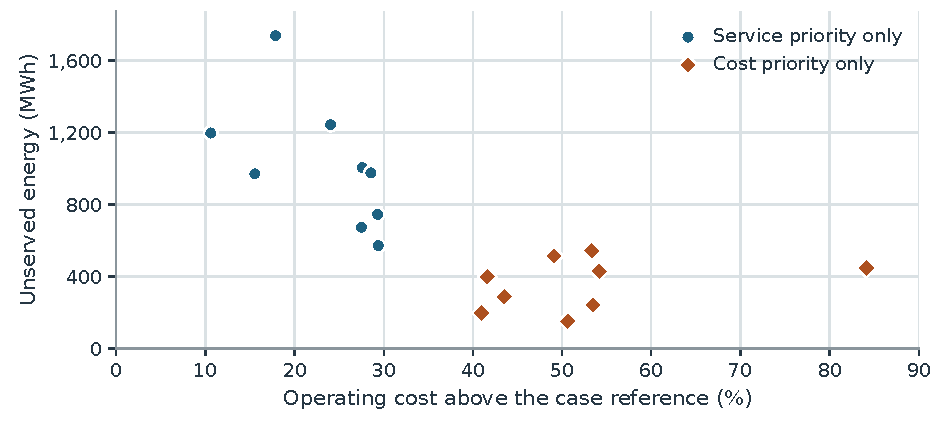
\includegraphics[width=.94\linewidth]{figures/vt_priority_shortlist.pdf}
\caption{The 18 cases on which the service and cost lists disagree. Each point is a delivered schedule at 120 seconds. A case can also appear on any of the other three lists. Unserved energy is the daily total in MWh. Cost overrun is measured relative to the absolute value of that case's strengthened reference cost. The 51 cases common to both lists are omitted.}
\label{fig:shortlist}
\end{figure}

\begin{table}[H]\centering\small\setlength{\tabcolsep}{3.2pt}
\caption{Development cases selected exclusively under the service or cost priority at 120 seconds, using the strengthened references.}\label{tab:exclusive_cases}
\begin{tabular}{@{}lrrrrrrrrrr@{}}\toprule
 & \multicolumn{2}{c}{Rank} & \multicolumn{2}{c}{Score margin} & \multicolumn{2}{c}{Unserved} & \multicolumn{2}{c}{Cost excess} & Time & Thermal\\
Case & Service & Cost & Service & Cost & MWh & \% & M EUR & \% & s & \%\\\midrule
\multicolumn{11}{@{}l}{\emph{Service only}}\\
H-00009 & 34 & 74 & +43.9 & -43.4 & 1,738 & 0.200 & 10.46 & 17.87 & 84.3 & 6.46\\
D-00015 & 38 & 68 & +36.0 & -19.5 & 1,243 & 0.170 & 19.44 & 24.04 & 84.3 & 5.59\\
D-00012 & 41 & 62 & +29.0 & -5.2 & 1,005 & 0.134 & 26.20 & 27.58 & 84.3 & 11.43\\
D-00086 & 48 & 64 & +13.9 & -9.6 & 975 & 0.111 & 17.80 & 28.56 & 84.3 & 7.24\\
H-00008 & 50 & 87 & +10.4 & -110.9 & 1,197 & 0.160 & 7.28 & 10.60 & 84.3 & 4.36\\
N-00030 & 55 & 65 & +4.0 & -11.7 & 744 & 0.095 & 6.81 & 29.31 & 84.3 & 5.28\\
D-00007 & 56 & 63 & +3.0 & -8.4 & 571 & 0.084 & 15.86 & 29.38 & 82.6 & 10.80\\
H-00013 & 57 & 82 & +1.4 & -70.7 & 970 & 0.123 & 9.89 & 15.54 & 82.7 & 3.93\\
D-00038 & 59 & 69 & +0.2 & -19.6 & 673 & 0.096 & 16.30 & 27.49 & 82.6 & 4.27\\
\addlinespace
\multicolumn{11}{@{}l}{\emph{Cost only}}\\
D-00059 & 61 & 40 & -1.3 & +39.4 & 447 & 0.059 & 12.65 & 84.13 & 84.3 & 6.58\\
D-00065 & 68 & 48 & -19.9 & +20.7 & 241 & 0.027 & 35.07 & 53.44 & 84.4 & 8.99\\
H-00063 & 63 & 51 & -4.5 & +18.4 & 543 & 0.068 & 5.05 & 53.32 & 84.4 & 2.88\\
D-00023 & 64 & 52 & -12.2 & +16.1 & 428 & 0.057 & 33.88 & 54.16 & 82.7 & 3.09\\
D-00034 & 62 & 53 & -4.4 & +15.7 & 514 & 0.067 & 34.67 & 49.09 & 84.2 & 4.13\\
H-00074 & 73 & 54 & -30.0 & +12.5 & 151 & 0.018 & 4.52 & 50.65 & 84.3 & 5.22\\
D-00052 & 66 & 55 & -16.2 & +9.3 & 288 & 0.042 & 31.78 & 43.50 & 84.2 & 6.70\\
D-00035 & 65 & 56 & -13.3 & +8.1 & 398 & 0.048 & 35.18 & 41.59 & 84.3 & 7.20\\
H-00047 & 72 & 58 & -29.7 & +0.8 & 196 & 0.025 & 8.63 & 40.96 & 84.3 & 4.16\\
\bottomrule\end{tabular}
\par\smallskip\begin{minipage}{\linewidth}\footnotesize
H denotes the high-criticality family, D the discrete-decision family and N the network family. The number is the case identifier within its family. Rank 1 has the largest loss. Each margin is the case's score minus its profile's 60th-highest score, multiplied by 1,000. A positive margin places the case inside the shortlist. Unserved energy is also expressed as a percentage of demand. Cost excess is the dispatch cost minus its reference, expressed in millions of euros and as a percentage of the absolute reference cost. Thermal is internal thermal generation as a percentage of served energy.
\end{minipage}\end{table}

\begin{table}[H]\centering\small
\caption{Median profile loss among development cases that delivered a valid dispatch.}\label{tab:conditional_loss}
\begin{tabular}{@{}rrrrrrr@{}}\toprule
Deadline (s) & Delivered & Service & Cost & Time & Emissions & Balanced\\\midrule
5 & 132 & 0.067 & 0.067 & 0.285 & 0.101 & 0.126\\
10 & 311 & 0.128 & 0.130 & 0.557 & 0.139 & 0.240\\
30 & 594 & 0.105 & 0.107 & 0.462 & 0.116 & 0.197\\
60 & 600 & 0.090 & 0.090 & 0.393 & 0.101 & 0.169\\
120 & 600 & 0.046 & 0.046 & 0.200 & 0.071 & 0.087\\
\bottomrule\end{tabular}
\par\smallskip\begin{minipage}{\linewidth}\footnotesize
All five profiles evaluate the same deliveries at each deadline. The set of delivered cases changes with the deadline. Each row uses the strengthened references. The initial references give the same medians to the precision shown.
\end{minipage}\end{table}

\paragraph{Feasible alternatives to the delivered schedules.}
Direct optimisation missed ES at all five deadlines in 125 cases. The initial reference dispatch met the strengthened cost and service criteria for 123. Including the longer reference runs raised this count to 124.
For the remaining case, N-00039, a different scheduling method delivered a physically validated dispatch in 115.2 seconds. It left zero MWh unserved and cost 3.52\% more than the strengthened reference. An acceptable dispatch is therefore documented for each of the 125 cases.

\section{Predicting loss on the development benchmark}
\label{app:devfit}
The fixed index spans 0.293--0.525 on these 600 cases. Giving all weight to the physical block reverses the order of 28.4\% of case pairs compared with the equal-block index. Giving all weight to the structural block reverses 13.4\%. At 120 seconds the original ES Brier score falls from 0.1084 for size alone to 0.0969 when the index is added and 0.0726 with the six selected generator indicators. The six count variables used in the independent test are a different set.

Tables~\ref{tab:mse} and \ref{tab:weights} use the original development costs. Allowing weights to vary across deadlines improves on varying the overall slope alone in 23 of 25 profile--deadline comparisons with positive lower bounds in the simultaneous intervals. The associations of individual indicators are less precisely known. For the emissions profile at 120 seconds, the fitted share for thermal density is 33.3\% (pointwise 95\% refit interval 27.6--41.6\%). For the nominal discrete decision count it is 30.5\% (19.3--41.8\%). The overlaps caution against interpreting the order of these two point estimates as a physical ranking of importance.


\begin{table}[H]\centering\tablefont
\caption{Prediction error for each profile. The first four columns of results show MSE on held-out scenarios from represented families. The last column evaluates the deadline-specific weights with an entire family withheld. Each cell pools 600 scenarios and five deadlines. Compare errors within a row because each profile defines its own response.}\label{tab:mse}
\begin{tabular}{@{}lrrrrr@{}}\toprule
& \multicolumn{4}{c}{Scenario held out} & Family held out\\
\cmidrule(lr){2-5}\cmidrule(l){6-6}
Priority & \shortstack{Reference\\index} & \shortstack{Common\\weights, slope} & \shortstack{Common weights,\\varying slope} & \shortstack{Varying weights\\and slope} & \shortstack{Varying weights\\and slope}\\\midrule
Service       & .04469 & .03739 & .02385 & .01728 & .05152\\
Cost          & .05506 & .03985 & .03443 & .02371 & .08601\\
Time          & .02446 & .01550 & .01366 & .00873 & .03158\\
Direct \CO    & .04438 & .03855 & .02315 & .01753 & .04771\\
Equal         & .03646 & .02767 & .02000 & .01353 & .04310\\
\bottomrule\end{tabular}
\end{table}

\begin{table}[H]\centering\tablefont
\caption{Largest fitted indicator shares by profile. Entries show the indicator code and its percentage of the total slope. A1 is the wind and solar share, A6 the peak-to-firm ratio, B1 zone count, B3 the discrete decision estimate, B4 thermal units per zone and B9 potential links per zone. Numbers are descriptive point estimates from all 600 historical scenarios.}\label{tab:weights}
\begin{tabular}{@{}lrrlll@{}}\toprule
& \multicolumn{2}{c}{Leading indicator} & \multicolumn{3}{c}{Three largest weights at 120 s}\\
\cmidrule(lr){2-3}\cmidrule(l){4-6}
Priority & 5 s & 30 s & First & Second & Third\\\midrule
Service & A1 (19.1) & B3 (57.6) & B3 (30.9) & B4 (27.8) & B9 (20.9)\\
Cost    & A1 (19.9) & B3 (53.0) & B3 (28.3) & B9 (27.7) & B4 (22.9)\\
Time    & A1 (24.1) & B1 (37.8) & B4 (34.3) & B3 (32.5) & A6 (27.7)\\
Direct \CO & A1 (17.6) & B3 (49.2) & B4 (33.3) & B3 (30.5) & B9 (21.2)\\
Equal   & A1 (20.3) & B3 (53.1) & B3 (35.0) & B4 (28.3) & B9 (18.3)\\
\bottomrule\end{tabular}
\end{table}

Across 48 combinations of priorities, anchors and cost definitions, the pooled error gain from deadline-specific weights remains positive. In a separate development analysis on constructed inputs, a bounded regression refitted without lines per zone reduces MSE by 19--31\% in scenario splits and 38--61\% in family holdouts relative to the clipped linear regression on the full constructed set. That refit was exploratory. Only the frozen linear and logistic models were evaluated on the independent cases in Table~\ref{tab:final_independent_descriptors}.


\section{Review quotas and the cost of omissions}
\label{app:selection}
Within each test portfolio, the review quota specifies the number $k$ of cases to examine. Recall is the fraction of the $k$ highest observed losses that the forecast selects. Mean selection regret is the average observed loss in the retrospective top $k$ minus the average observed loss in the forecast top $k$. Zero regret means the selected list captures the full loss available for review at that quota. We resolve ties using an ordering derived from case identifiers independently of measured outcomes. The uniform comparator uses its expected overlap and mean selected loss. Original development costs gave 28, 26, 36, 28 and 33 hits (service, cost, time, emissions and balanced) with tailored forecasts at the 10\% quota. Table~\ref{tab:review} reports the strengthened costs applied to those same forecasts. These analyses use unprojected forecasts at the 120-second deadline and were specified after the main tests.

\begin{table}[htbp]\centering\small
\caption{Priority cases recovered at three review quotas. Ranges give the lowest and highest recall (percent) across the five mandates. Development uses strengthened references and five held-out portfolios of 120. The independent test uses four batches of 100. In the zone-count rule the largest systems receive priority.}
\begin{tabular}{@{}lrrr rrr@{}}\toprule
& \multicolumn{3}{c}{Development} & \multicolumn{3}{c}{Independent test}\\
\cmidrule(lr){2-4}\cmidrule(l){5-7}
Selection rule & 5\% & 10\% & 20\% & 5\% & 10\% & 20\%\\\midrule
Mandate-specific, 22 indicators & 7--43 & 43--62 & 73--77 & 15--20 & 18--40 & 35--64\\
Balanced, 22 indicators & 27 & 50--55 & 74--76 & 15 & 23--33 & 36--58\\
Zone count & 7--10 & 27--32 & 56--58 & 10 & 25--38 & 33--54\\
Three constructed measures & \multicolumn{3}{c}{---} & 20--25 & 23--30 & 31--51\\
Six model counts & \multicolumn{3}{c}{---} & 15--20 & 23--33 & 34--56\\
Uniform, expected & 5 & 10 & 20 & 5 & 10 & 20\\
\bottomrule\end{tabular}
\end{table}

For the independent time-priority score at the 10\% quota, tailoring reduced regret from 0.186 to 0.128 on the unit loss scale. The paired difference was $-0.0585$ (pointwise 95\% interval $[-0.115,-0.007]$, with 2,000 within-batch resamples of cases and the lists rebuilt for each resample). The corresponding intervals for the cost, service and emissions priorities included zero. Among 30 independent service-priority cases missed by the tailored forecast, ten exceeded the service tolerance and the largest shortfall was 3,501 MWh. When we refit the models under alternative scoring assumptions using the original development reference costs, tailoring reduced regret at the 10\% quota for nine of ten time-priority specifications. It increased regret for all ten specifications for each of the service, cost and emissions priorities.

\section{Comparing representations on the independent test}
\label{app:external}

\begin{table}[htbp]\centering\tablefont
\caption{Independent prediction error multiplied by 1,000. Smaller values are better within each row. The five profile rows give MSE after bounding predictions to $[0,1]$. E and ES give Brier scores. Each cell averages 400 cases at five deadlines.}
\label{tab:final_independent_descriptors}
\begin{tabular}{@{}lrrrrr@{}}\toprule
& \multicolumn{3}{c}{22 indicators} & \multicolumn{2}{c}{Compact sets}\\
\cmidrule(lr){2-4}\cmidrule(l){5-6}
Target & Generator & MILP & MILP, B9 limited & Three measures & Six counts\\\midrule
Balanced & 44.35 & 52.75 & 45.73 & 35.25 & \textbf{29.23}\\
Service priority & 47.38 & 60.54 & 51.86 & 39.80 & \textbf{35.65}\\
Cost priority & 55.56 & 63.32 & 55.46 & 41.79 & \textbf{34.27}\\
Time priority & 43.07 & 73.52 & 42.00 & 38.31 & \textbf{31.14}\\
Direct \CO{} priority & 46.01 & 58.65 & 50.42 & 39.62 & \textbf{35.50}\\
\addlinespace
Economic success (E) & 83.38 & 145.27 & 86.28 & \textbf{59.93} & 66.27\\
Joint success (ES) & 128.72 & 131.52 & 132.02 & \textbf{98.00} & 107.86\\
\bottomrule\end{tabular}
\end{table}

Here the generator and MILP columns use the raw indicators standardized on development data. The three measures are zones, free binary variables and the fraction of zones with thermal capacity. The six counts are zones, time steps, lines, variables, free binary variables and constraints included before solving. The B9-limited column changes only lines per zone when outside its training range. All coefficients stay frozen. Bold type identifies the lowest point estimate in each row.

The three measures improve on the 22 generator indicators for each of the five profile scores, with reductions in projected MSE of 11.1--24.8\%. For the comparison between the two full sets, the projected average balanced-score error difference (MILP minus generator) is 0.00840, with a simultaneous 95\% interval of 0.00268 to 0.01412. For ES the difference is 0.00280, with an interval of $-0.01174$ to 0.01735. The five continuous scores favour the generator set in this pooled comparison. The relative ordering in each of the seven full-set comparisons is the same on restricting the test to the 389 cases with certified references. The raw forecasts by batch and deadline were prespecified. Pooling the batches, bounding the output and examining B9 were subsequent diagnostics.

\begin{figure}[H]
\centering
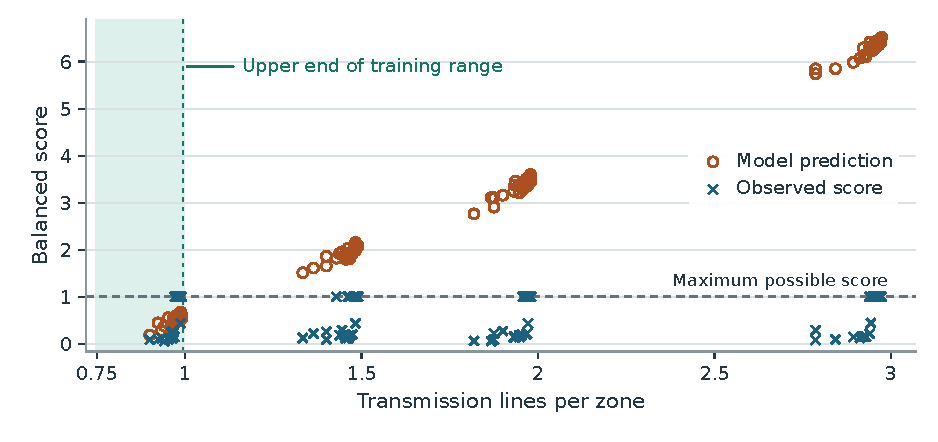
\includegraphics[width=.94\linewidth]{figures/vt_topology_transfer.pdf}
\caption{Predicting the balanced score on unfamiliar networks. Each of the 100 cases is shown twice, with its observed score and its five-second forecast from the model using 22 measurements of the scheduling problem. Shading marks the range of lines per zone in training.}
\label{fig:transfer}
\end{figure}

\paragraph{Secondary comparisons.}
With all forecasts left unadjusted, pooled errors across the five deadlines ranged from 0.408 to 0.659 for the 22 constructed-system measures and from 0.043 to 0.056 for the 22 generator indicators, depending on the profile. On the unfiltered batch, the constructed-system measures improved all five point estimates after bounding the forecasts. For the balanced score, their error was 0.0313 compared with 0.0341 for the generator set. In the altered-topology batch the corresponding errors were 0.0720 and 0.0415. Across the independent sample, limiting only lines per zone to its observed training range and bounding the output reduced balanced-score error from 0.0528 to 0.0457, closing 84\% of the gap to the generator set. For the joint success probability this intervention slightly worsened the Brier score. These are comparisons between forecasts. Inferring what would happen to dispatch if an individual line were added would require a separate physical comparison.

\section{Selecting days on a fixed grid}
\label{app:fixeddays}

\paragraph{Design.}
We selected the first numbered network in the medium-difficulty family before running the experiment. Its 56 zones and 55 lines, plant capacities, costs, hydro inflows and initial storage stayed fixed. Each synthetic day starts from the same initial conditions and spans 24 hours. We draw one of four demand patterns (flat, evening peak, double peak or office-hours peak), give it equal weight with each zone's original pattern, and scale the resulting peak to 75--125\% of that zone's original peak. The hourly wind and solar series combine a regional weather pattern (75\% weight) with the zone's original availability (25\%). We then scale solar availability by a factor drawn from 0.40--1.00 and wind availability by a factor drawn from 0.35--1.00. The share of demand that can be shifted stays fixed.

We set the daily inputs and selection rules and applied the fitted forecasts before solving. Each day had two timed runs and a separate reference run with a 600-second solver limit. All 60 timed runs delivered valid plans on time. All 30 reference runs delivered feasible plans, and the solver certified four as optimal within tolerance. Reported cost overruns use each day's feasible reference. At 30 seconds, 24 plans met the cost requirement and 22 also met the service requirement. The corresponding counts at 120 seconds were 28 and 28.

\paragraph{Selection and uncertainty.}
Each rule selects six of the 30 days separately at each deadline. For a tie at the cutoff we give tied days equal chances of taking the remaining places. A rule that ties all days therefore finds \(6\times6/30=1.2\) of the six highest-scoring days on average. For each priority and deadline we also compare the mean observed score of the six highest-scoring days with that of the six selected in advance. Their difference is the \emph{selection regret}, the primary measure specified for this pilot. Zero means the selection captures the highest possible average score. A small difference means it captures much of the severity even if some days differ.

\begin{table}[htbp]\centering\tablefont
\caption{How far did each selection fall short of the six most concerning days? Entries give selection regret in score units on the zero-to-one scale. Smaller values are better within a column at a given deadline.}
\label{tab:fixed_regret}
\begin{tabular}{@{}llrrrrr@{}}\toprule
Deadline & Selection rule & Service & Cost & Time & Emissions & Balanced\\\midrule
30 s & Random selection & 0.075 & 0.331 & 0.070 & 0.049 & 0.130\\
 & Highest residual peak & 0.095 & 0.441 & 0.089 & 0.038 & 0.164\\
 & Largest hourly rise & 0.069 & 0.292 & 0.065 & 0.049 & 0.117\\
 & 22 measures & 0.088 & 0.367 & 0.090 & 0.056 & 0.170\\
\addlinespace
120 s & Random selection & 0.031 & 0.146 & 0.048 & 0.039 & 0.058\\
 & Highest residual peak & 0.052 & 0.198 & 0.139 & 0.031 & 0.097\\
 & Largest hourly rise & 0.023 & 0.121 & 0.022 & 0.037 & 0.043\\
 & 22 measures & 0.056 & 0.202 & 0.143 & 0.049 & 0.104\\
\bottomrule\end{tabular}
\end{table}

The forecasts based on three structural measures or six counts, and the rule using initial stored energy, each tied all days and had the same regret as random selection. Another rule ranks days by the smallest supply margin at the residual peak. This margin is thermal and nuclear capacity plus available run-of-river hydroelectric output at the peak, less residual load. It selected the same six days as the peak rule. The 22-measure forecasts used the fitted coefficients from the earlier study and were bounded to the score range before ranking.

For the balanced perspective at two minutes, selecting the largest hourly rises reduced regret from 0.058 under random selection to 0.043 (Table~\ref{tab:fixed_regret}). The gain was 0.015 score units, with a 95\% interval from \(-0.010\) to \(0.060\). We obtained each interval by resampling the 30 days 1,000 times, comparing rules on the same sampled days and keeping fitted models fixed. Each interval describes a single comparison on this grid. It omits variation from repeating the solver runs.

\section{Allocation under alternative computing reserves}
\label{app:reserve}

\begin{table}[htbp]\centering\tablefont
\caption{Observed joint successes for each average computing reserve. Columns 10--60 give reserved seconds per case. At 20 seconds, the uniform rule assigns half the cases 10 seconds and half 30 seconds, in a fixed order independent of their outcomes. The other uniform rules assign the indicated time to every case.}
\label{tab:allreserves}
\begin{tabular}{@{}lrrrr rrrr@{}}\toprule
 & \multicolumn{4}{c}{Development (600)} & \multicolumn{4}{c}{Independent (400)}\\
\cmidrule(lr){2-5}\cmidrule(l){6-9}
Allocation rule & 10 & 20 & 30 & 60 & 10 & 20 & 30 & 60\\\midrule
Uniform & 168 & 265 & 341 & 430 & 253 & 307 & 351 & 366\\
Zone count & 231 & 344 & 395 & 451 & 248 & 331 & 352 & 370\\
Reference index & 218 & 322 & 378 & 450 & 235 & 307 & 347 & 373\\
Three generator indicators & 256 & 364 & 413 & 464 & 259 & 345 & 362 & 370\\
22 normalized generator indicators & 249 & 359 & 415 & 459 & 244 & 335 & 350 & 370\\
Three constructed measures & \multicolumn{4}{c}{---} & 267 & 342 & 353 & 361\\
Six model counts & \multicolumn{4}{c}{---} & 266 & 346 & 353 & 361\\
22 constructed measures & \multicolumn{4}{c}{---} & 242 & 309 & 344 & 363\\
Hindsight & 273 & 417 & 472 & 475 & 312 & 370 & 374 & 374\\
\bottomrule\end{tabular}
\end{table}

This retrospective analysis allocates a separate reserve to each held-out development portfolio or independent batch. Within a portfolio, a discrete optimisation chooses exactly one of the five deadlines for every case. Its objective is the sum of the corresponding predicted probabilities of ES. For the hindsight rule, we assign one to a case and deadline if its observed schedule met both requirements and zero otherwise. The allocation cannot use seconds released early by a previous run. Thus the reserve is the sum of the deadlines offered, while actual run time is the sum of the recorded times to exit.

The independent replay uses frozen probabilities. We recomputed the allocation in 200 paired resamples of cases within the four batches, with predictors fixed. At 30 seconds the gain over uniform allocation is 11 cases for the nominal three-indicator rule (pointwise 95\% interval 6 to 18) and minus one for the normalized 22-indicator rule (interval $-6$ to 4). Table~\ref{tab:allreserves} reports gross reserves. This decision analysis was specified after the independent scores were examined.

We also charged the time to obtain inputs and allocate the independent reserve. For the generator indicators we timed the calculation from the scenario inputs. For the indicators measured from the scheduling model we timed the calculation after model construction. We also charged for construction if the model had to be built again for scheduling. In both cases we allowed one additional second per batch to apply the fitted forecasts and choose the deadlines. At 30 seconds per case the nominal trio still yields 362 successes and the full normalized generator set yields 350. The constructed trio and the six counts each yield 353 successes when the model is reused for scheduling and 352 when it is built twice. For example, when the three-indicator rule reuses the model, it reserves 11,940 of the available 12,000 seconds for scheduling. Measuring the indicators and assigning deadlines takes a further 20.47 seconds. The scheduling runs used 5,396 seconds in total, compared with 4,872 for uniform allocation. This calculation shows how much of the computing reserve is available for scheduling after measuring the indicators and choosing the deadlines.

\end{document}
